\documentclass[12pt]{article}

\usepackage{graphicx}
\usepackage{amsmath}
\usepackage{amssymb}
\usepackage{geometry}
\geometry{a4paper, margin=1in}

\title{Multi-Agent Systems HW6:\\Final Homework Assignment}
\author{Fei Huang, 2818760}
\date{\today}

\begin{document}

\maketitle

\section{Monte Carlo Simulation}

\subsection{Optimal Batch Size}

\subsubsection*{Objective}
The goal of this section is to use Monte Carlo simulation to estimate the optimal batch size \( k \) that minimizes the expected number of tests for a given value of \( p \) where \( p \) can take values between \( 10^{-1} \) and \( 10^{-4} \).

\subsubsection*{Methodology}

A Python function, \texttt{monte\_carlo\_simulation\_optimized}, was developed to simulate the batch testing process utilizing the Monte Carlo method. Given a population size \( N \) and a prevalence rate \( p \), this function iteratively calculates the average number of tests required for each batch size \(k\) within a defined range across multiple iterations, ensuring statistical validity. The batch size that minimizes the average number of tests is identified as the optimal batch size for the specified prevalence rate.

Furthermore, an in-depth analysis was performed across a spectrum of prevalence rates: 0.1, 0.01, 0.001, and 0.0001 to substantiate the results.

\subsubsection*{Results}

The Monte Carlo simulations reveal a pattern in the average number of tests required as a function of batch size \( k \) across different infection probabilities \( p \), and optimal batch sizes for each \( p \) are identified.

\begin{figure}[ht]
\centering
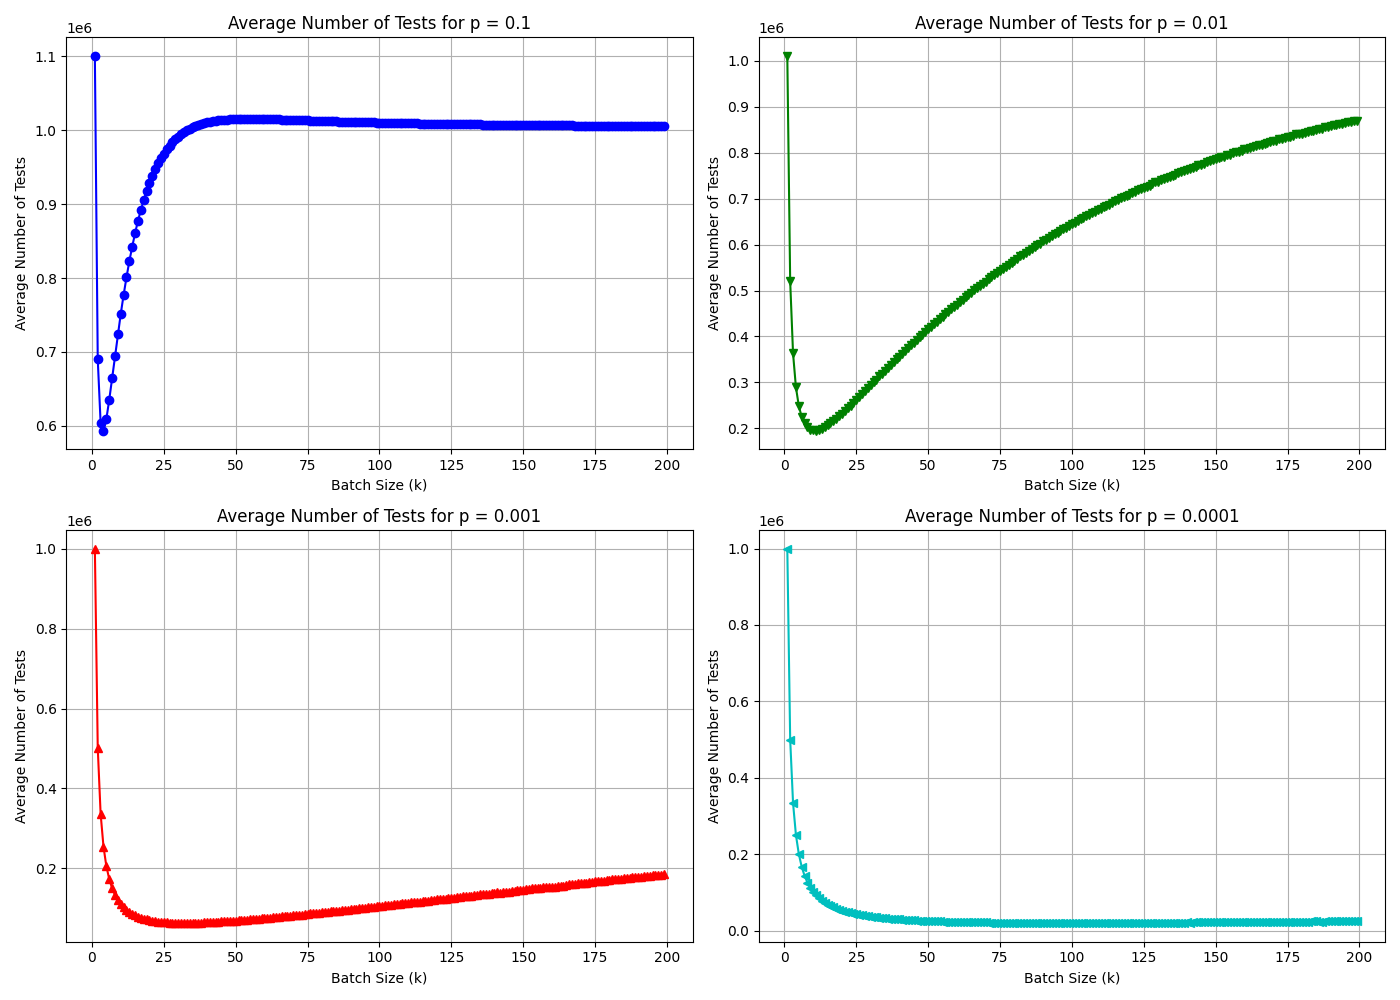
\includegraphics[width=0.8\textwidth]{image/1_MC_exploration.png}
\caption{Average number of tests as a function of batch size \( k \) for different \( p \) values.}
\end{figure}

For \( p = 0.01 \), as batch size \( k \) increases from 1, there is a significant decrease in the average number of tests. This decrease suggests that batch testing substantially reduces the total number of tests. The average number of tests reaches a minimum at a certain batch size, indicating an optimal point beyond which efficiency drops. At \( p = 0.01 \), the optimal batch size \( k \) is 11.

Similar trends are observed for other \( p \) values. With \( p = 0.1 \), the optimal batch size \( k \) is found to be smaller, at 4. For lower probabilities, \( p = 0.001 \) and \( p = 0.0001 \), the optimal batch sizes \( k \) are determined to be 32 and 107, respectively. 

\subsubsection*{Conclusion}

The findings suggest the existence of an optimal batch size \( k \) that minimizes the average number of tests, which varies with the infection probability \( p \). The optimal batch size increases with lower \( p \) and decreases with higher \( p \), highlighting the importance of adapting batch sizes to the expected infection rate to maximize testing efficiency.

\subsection{Expected Reduction in Tests}

\subsection*{Objective}
This section aims to quantify the expected reduction in the number of tests when using batch testing compared to individual testing.

\subsection*{Methodology}
To achieve this goal, a Python function named \texttt{calculate\_expected\_reduction} was developed, employing the existing Monte Carlo simulation method for the analysis.

The \texttt{calculate\_expected\_reduction} function utilizes the Monte Carlo method to simulate for each probability value \( p \) and batch size \( k \), calculating the average number of tests. This function further determines the optimal batch size for each \( p \) value and computes the expected reduction in the number of tests when using the optimal batch size compared to individual sample testing. This includes identifying the optimal batch size, calculating the average number of tests with the optimal batch, and determining the percentage reduction in tests compared to individual testing.

The analysis encompasses a range of prevalence rates logarithmically spaced from \( 10^{-1} \) to \( 10^{-4} \), consisting of 20 values. This selection of logarithmically spaced probabilities was made to ensure that our conclusions are more generalizable, reflecting trends and patterns across a broad spectrum of probabilities.

\subsection*{Results}

As observed in the Monte Carlo simulation, there is a significant inverse correlation between the prevalence rate \( p \) and the optimal batch size \( k \). This trend remains consistent across the entire range of prevalence rates examined, with the optimal batch size incrementally rising from 4 at \( p = 10^{-1} \) to 109 at \( p = 10^{-4} \).

\begin{figure}[ht]
\centering
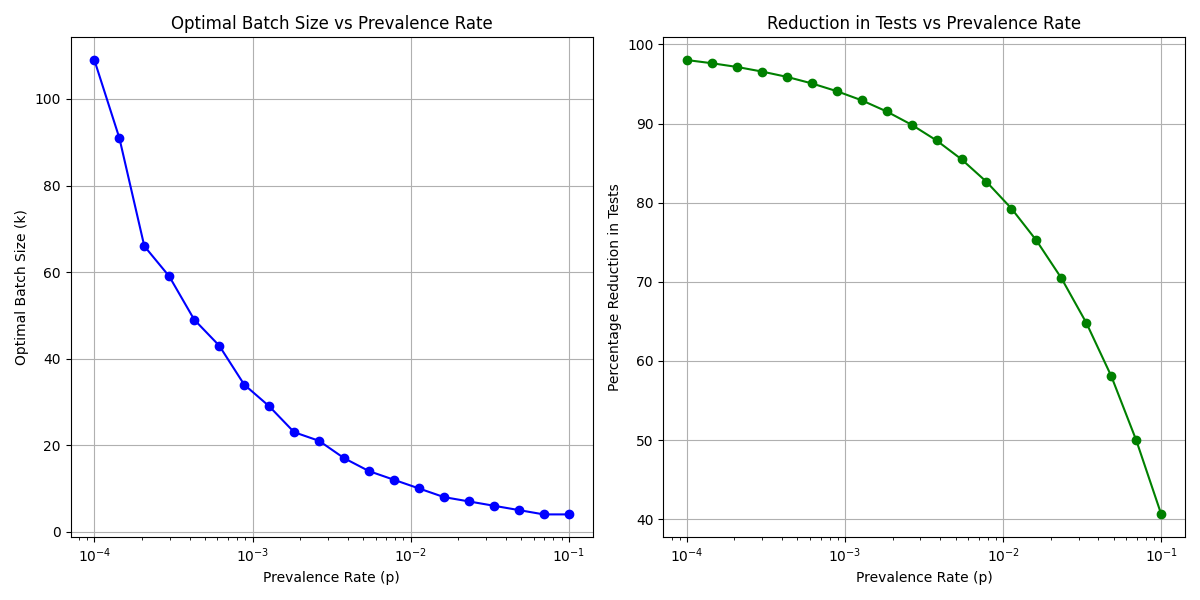
\includegraphics[width=0.8\textwidth]{image/1_OptimalSizeAndReduction.png}
\caption{Optimal Batch Size vs Prevalence Rate and Reduction in Tests vs Prevalence Rate.}
\end{figure}

The percentage reduction in tests underscores the effectiveness of the batch testing approach. With the application of the optimal batch size, a substantial reduction in the number of required tests is observed. The reduction commences at 40.61\% for a prevalence rate of \( p = 10^{-1} \) and escalates to an impressive 98.02\% for \( p = 10^{-4} \), emphasizing the scaling efficiency of batch testing as prevalence declines.

\subsection*{Conclusion}

The study indicates that batch testing can substantially reduce the number of tests required, particularly in low-prevalence scenarios. As the prevalence rate decreases, increasing batch sizes becomes more efficient. 

\section{Thompson Sampling for Multi-Armed Bandits}

\subsection{Objective}
The objective of this section is to apply the Thompson Sampling algorithm to the multi-armed bandit problem. The aim is to demonstrate, through simulation experiments, how Thompson Sampling progressively learns and optimizes the selection strategy over time to minimize regret.

\subsection{Methodology}
A simulation program was developed in Python, initializing two Beta distribution parameters \( \alpha \) and \( \beta \) both set to 1, representing the prior knowledge of the probability of success. Over 1000 iterations, these parameters were updated based on reward feedback, and the expected value and variance after each iteration were recorded. The methodology was also applied to a three-armed bandit problem, where over 3000 iterations, the selection process for three arms was simulated and the total regret was calculated.

\subsection{Results}
In the simulation of the single-armed bandit, the expected value was observed to gradually approach the true probability of success, while the variance progressively decreased. 

\begin{figure}[ht]
\centering
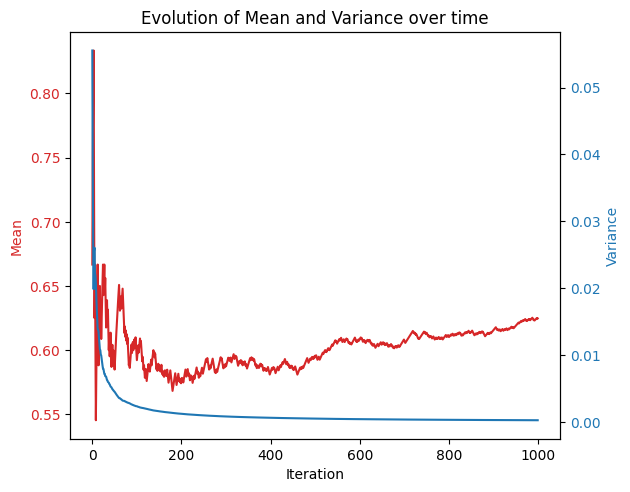
\includegraphics[width=0.8\textwidth]{image/2_OneArmedBandit.png}
\caption{Evolution of Mean and Variance over time for the single-armed bandit.}
\end{figure}

In the simulation of the three-armed bandit, Thompson Sampling demonstrated efficiency in selecting the best arm, with the speed of increase in total regret slowing over time, indicating an improvement in the decision-making process of the algorithm.

\begin{figure}[ht]
\centering
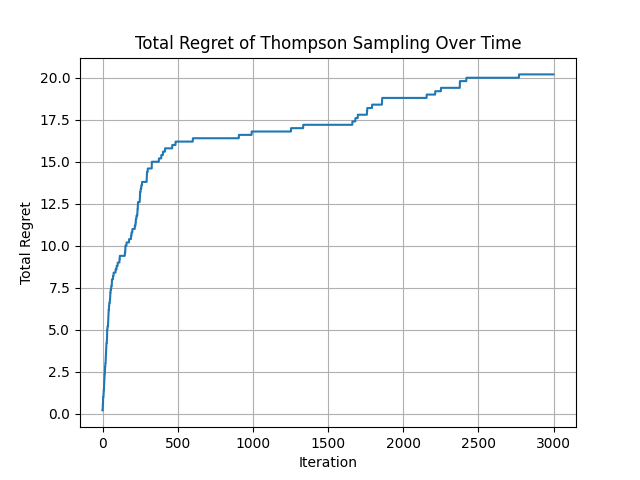
\includegraphics[width=0.8\textwidth]{image/2_ThreeArmedBandits.png}
\caption{Total Regret of Thompson Sampling Over Time for the three-armed bandit.}
\end{figure}

\subsection{Conclusion}
This study shows that Thompson Sampling is a useful method for solving multi-armed bandit problems. By continuously updating its strategy based on previous outcomes, it effectively minimizes regret over time. The simulations suggest that this approach is especially beneficial in situations where decisions must be made with incomplete information. 

\section{Reinforcement Learning: Cliff Walking}

\subsection{Objective}
The objective of this section is to investigate the Cliff Walking problem using reinforcement learning algorithms SARSA and Q-Learning. The aim is to compare the efficacy of these algorithms in navigating a path from a start state to a goal state while avoiding a cliff region that incurs a substantial negative reward.

\subsection{Methodology}

\subsubsection{Implementation}

A reinforcement learning framework was implemented in Python, which integrates an environment simulator, algorithmic agents, and an experimental management system. The \texttt{CliffWalkingEnv} class outlines the task's environmental parameters, establishing a grid-based simulation space with defined state transitions. Agents are constructed via the \texttt{Agent} class and are programmed to utilize either SARSA or Q-Learning algorithms for strategic navigation. The coordination of the learning sequence, along with the compilation of performance data and the depiction of the agents' policy evolution, is systematically conducted by the \texttt{Experiment} class.


\textbf{Environment Setup:} The Cliff Walking task is formalized as a grid-world environment, represented by the \texttt{CliffWalkingEnv} class. The environment has a predefined width and height, with designated start (S) and goal (G) states. A cliff region, which spans a contiguous set of states and imposes a severe negative reward upon entry, is explicitly defined. An optional snake pit can also be included to increase the task's complexity.

\textbf{Agent Implementation:}
The agents are instantiated through the \texttt{Agent} class, which is equipped with various learning strategies: SARSA and Q-Learning. Each agent has a state-size and action-size corresponding to the environment's dimensions and possible actions, respectively. The class also includes methods for choosing actions based on an epsilon-greedy policy and learning from the environment's feedback.

\textbf{Learning and Adaptation:}
The agents' learning mechanisms are realized through iterative updates to their action-value function (Q). For SARSA, the updates are done using the current and next actions, whereas Q-Learning utilizes the maximum value of the next state's actions. 

\textbf{Experience Replay:}
To enhance the Q-Learning agent's performance, a \texttt{ReplayBuffer} class was incorporated to store and sample experiences. This allows the agent to learn from a diverse set of past transitions, improving the stability and efficiency of the learning process.

\textbf{Experimentation Framework:}
The experimentation framework, encompassed within the \texttt{Experiment} class, coordinates the training process over a specified number of episodes. It manages the interaction between the agent and the environment, the accumulation of rewards, and the application of the learning algorithm. Additionally, the class provides methods for plotting the learning curve and visualizing the best route discovered by the agent.

\textbf{Route Visualization:}
A method within the \texttt{Experiment} class, \texttt{showRoute}, was developed to graphically display the route taken by the agent. This method plots the environment's grid, marks the start and goal states, and visually distinguishes the cliff, and the path taken by the agent.

\textbf{Statistical Evaluation:}
The training process's effectiveness is statistically evaluated by examining the average rewards obtained during the last ten episodes. This provides an indication of the agent's performance after having learned from the environment.
%
\subsubsection{Experimental Design}

\textbf{Parameter Selection:}
Given that the learning task is a standard, undiscounted, episodic task, the discount factor (\(\gamma\)) is inherently set to 1. In determining the appropriate learning rate (\(\alpha\)), initial experiments were conducted. It was observed that a higher \(\alpha\) makes the learning process disproportionately influenced by new samples. Additionally, as the learning rate is not the central subject of this research, a fixed value of \(\alpha = 0.1\) was selected. The exploration rate (\(\epsilon\)) was set to 0.1 by default.

\textbf{Study Design:}
The first set of experiments involved testing both SARSA and Q-Learning algorithms, implemented with and without a replay buffer. Subsequent experiments were conducted with varying levels of \(\epsilon\), specifically lower and higher values, to assess their effects on the learning process. Finally, the complexity of the environment was increased by introducing a snake pit, aiming to evaluate the robustness of the learning strategies in more challenging scenarios.


\subsection{Results}

\subsubsection{Comparison of Different Strategies}
The experiments involving SARSA and Q-Learning algorithms exhibited distinct learning behaviors. A comparison of learning curves and optimal paths under default settings revealed that SARSA tended to favor safer paths, while Q-Learning was inclined towards more optimal but riskier paths. SARSA demonstrated a consistent learning curve with gradual improvement in path efficiency. In contrast, Q-Learning showed rapid initial learning, but its subsequent variance in performance was notably higher than SARSA.

\begin{figure}[ht]
    \centering
    \begin{minipage}[b]{0.48\textwidth}
        \centering
        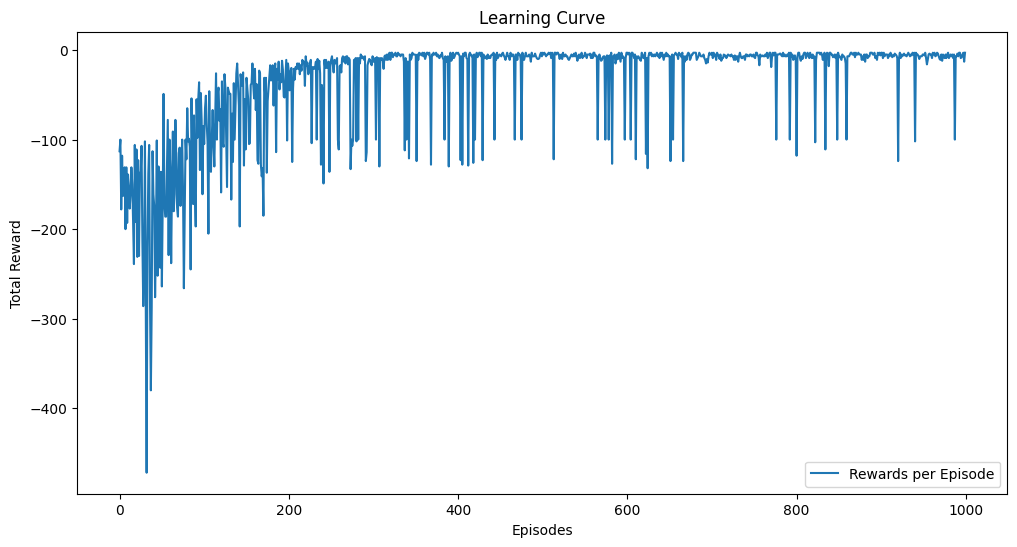
\includegraphics[width=\textwidth]{image/L1.1.png}
        \caption{\scriptsize Learning curves for SARSA with \(\epsilon=0.1\)}
        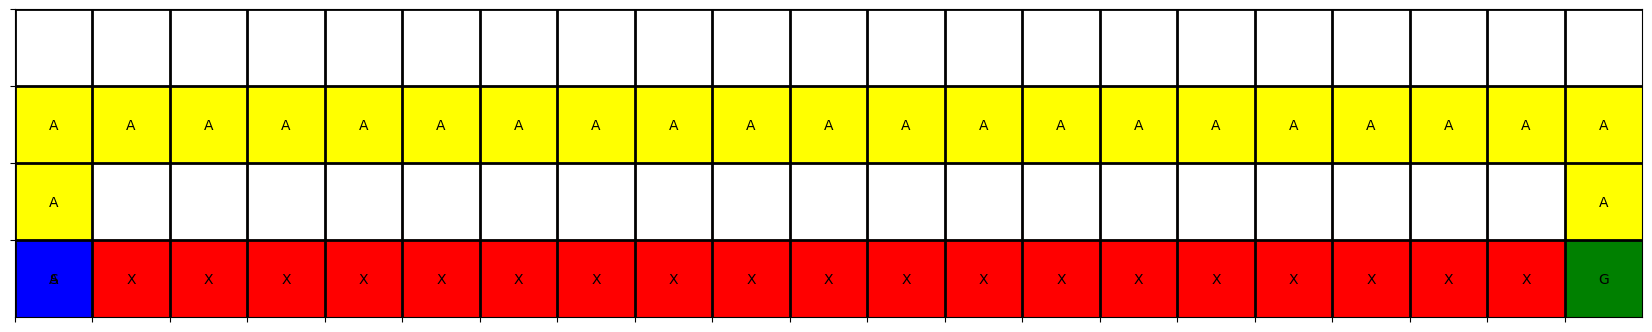
\includegraphics[width=\textwidth]{image/R1.1.png}
        \caption{\scriptsize Optimal path under SARSA with \(\epsilon=0.1\)}
    \end{minipage}
    \hfill
    \begin{minipage}[b]{0.48\textwidth}
        \centering
        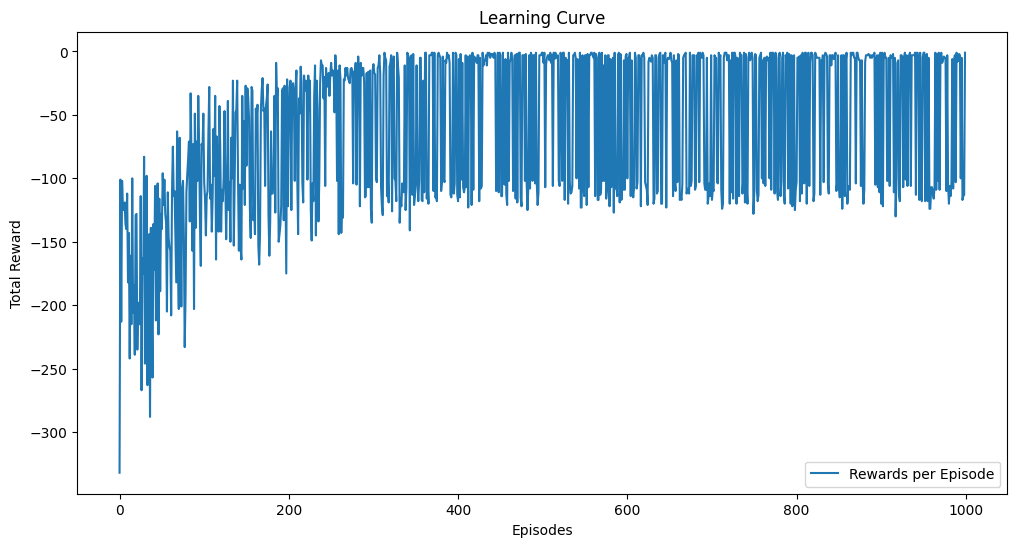
\includegraphics[width=\textwidth]{image/L1.2.png}
        \caption{\scriptsize Learning curves for Q-Learning(with replay-buffer) and \(\epsilon=0.1\)}
        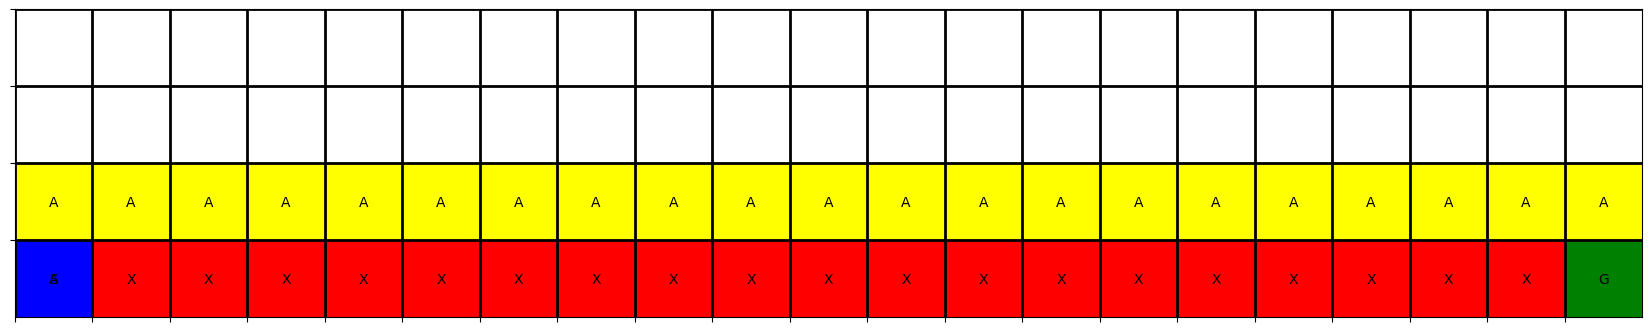
\includegraphics[width=\textwidth]{image/R1.2.png}
        \caption{\scriptsize Optimal path under Q-Learning(with replay-buffer) and \(\epsilon=0.1\)}
    \end{minipage}
\end{figure}

\subsubsection{Impact of Different Exploration Rates}
Exploration rate variations had a negligible effect on the optimal path learned by Q-Learning. For SARSA, however, a lower exploration rate steered the algorithm towards more optimal paths, while a higher rate favored safer paths. The impact of exploration rates on learning curves was significant and consistent across both algorithms. Lower exploration rates led to quicker convergence and less fluctuation, whereas higher rates resulted in slower convergence and greater variance.

\begin{figure}[ht]
    \centering
    \begin{minipage}[b]{0.48\textwidth}
        \centering
        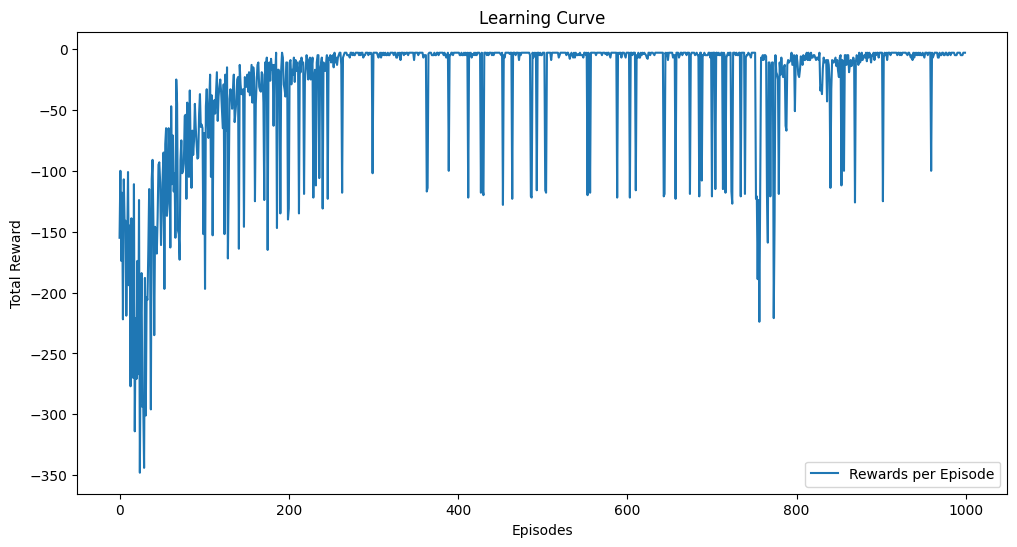
\includegraphics[width=\textwidth]{image/L2.1.png}
        \caption{\scriptsize Learning curves for SARSA with \(\epsilon=0.03\)}
        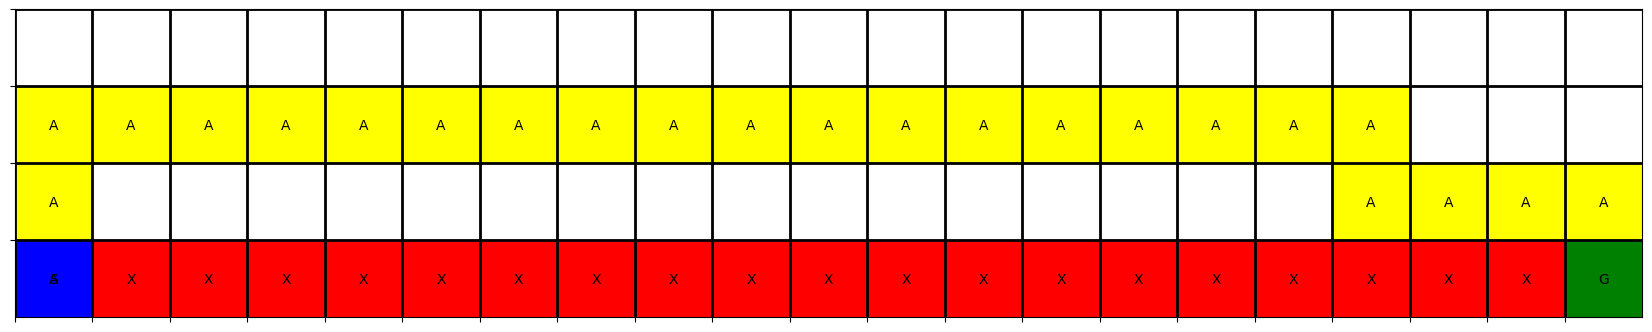
\includegraphics[width=\textwidth]{image/R2.1.png}
        \caption{\scriptsize Optimal path under SARSA with \(\epsilon=0.03\)}
    \end{minipage}
    \hfill
    \begin{minipage}[b]{0.48\textwidth}
        \centering
        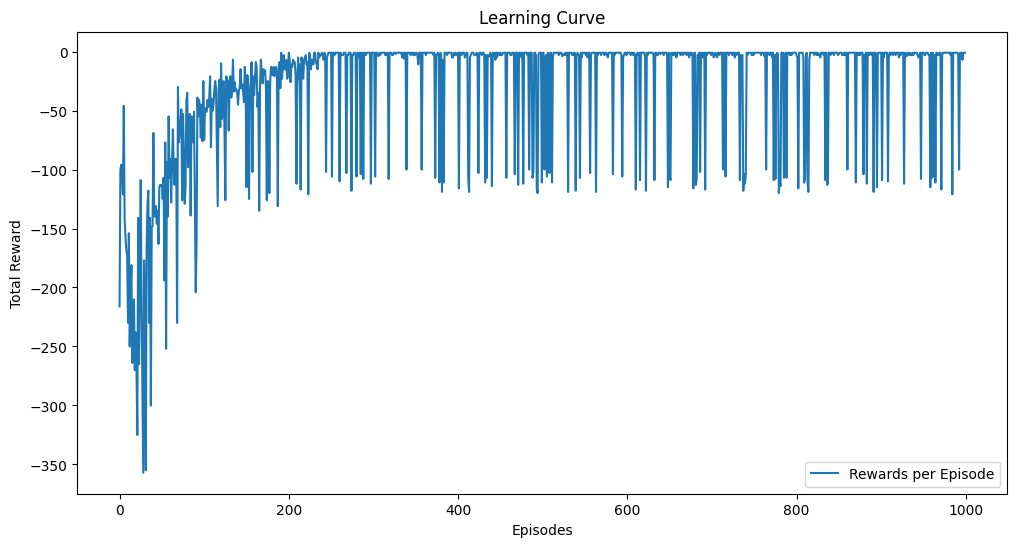
\includegraphics[width=\textwidth]{image/L2.3.png}
        \caption{\scriptsize Learning curves for Q-Learning \(\epsilon=0.03\)}
        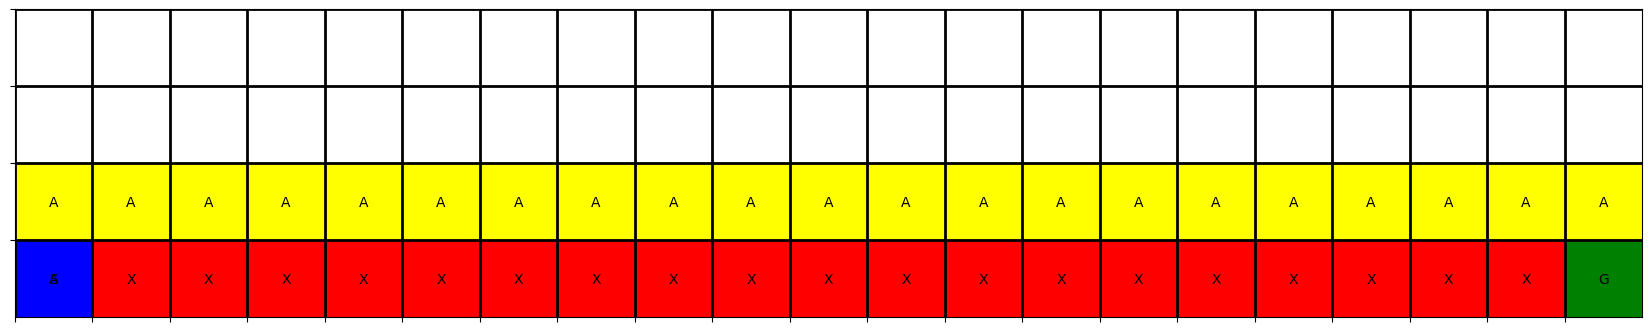
\includegraphics[width=\textwidth]{image/R2.3.png}
        \caption{\scriptsize Optimal path under Q-Learning \(\epsilon=0.03\)}
    \end{minipage}
\end{figure}

\begin{figure}[ht]
    \centering
    \begin{minipage}[b]{0.48\textwidth}
        \centering
        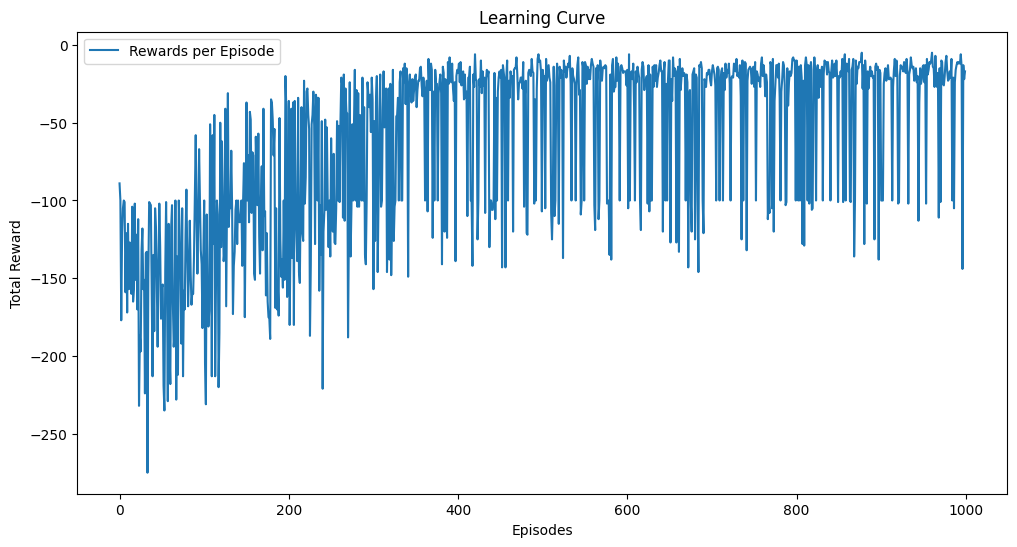
\includegraphics[width=\textwidth]{image/L2.2.png}
        \caption{\scriptsize Learning curves for SARSA with \(\epsilon=0.3\)}
        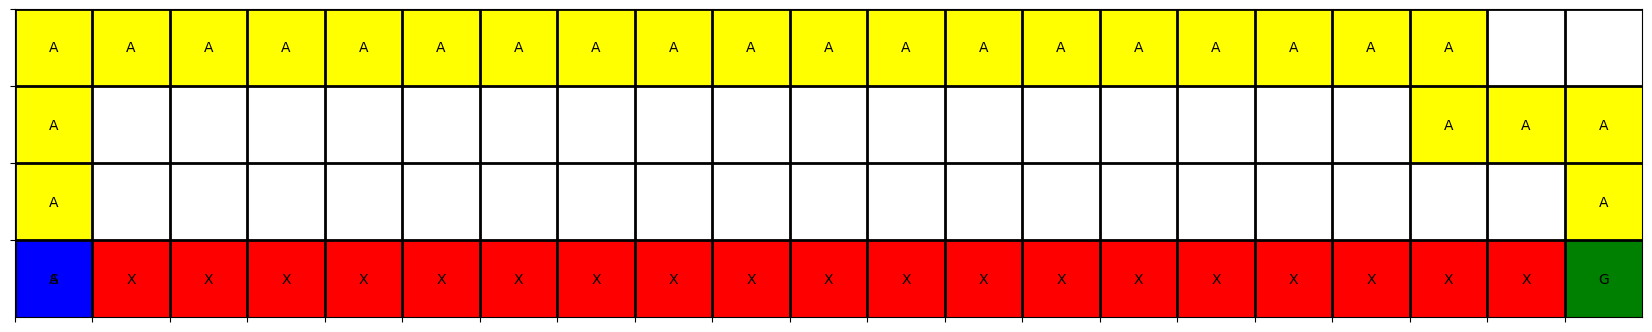
\includegraphics[width=\textwidth]{image/R2.2.png}
        \caption{\scriptsize Optimal path under SARSA with \(\epsilon=0.3\)}
    \end{minipage}
    \hfill
    \begin{minipage}[b]{0.48\textwidth}
        \centering
        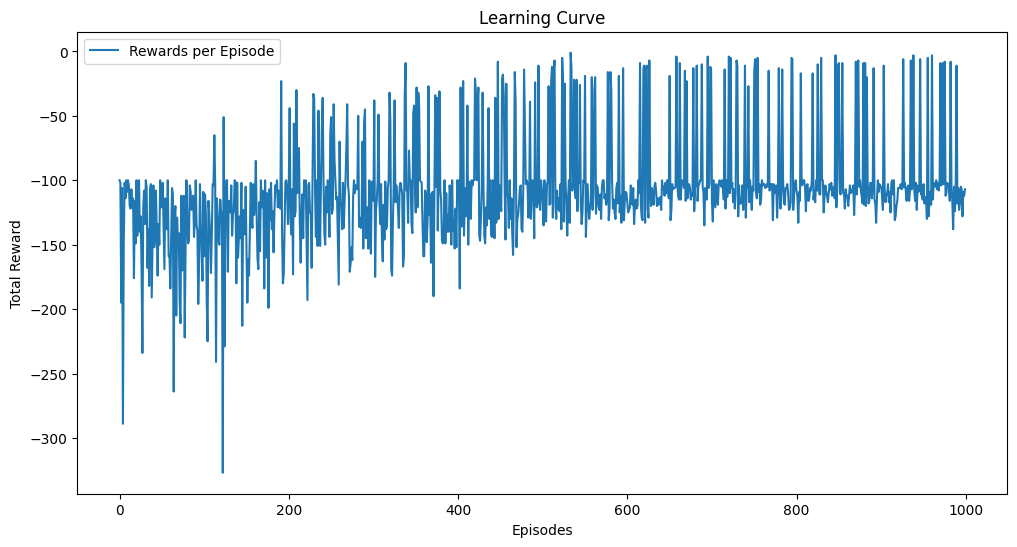
\includegraphics[width=\textwidth]{image/L2.4.png}
        \caption{\scriptsize Learning curves for Q-Learning \(\epsilon=0.3\)}
        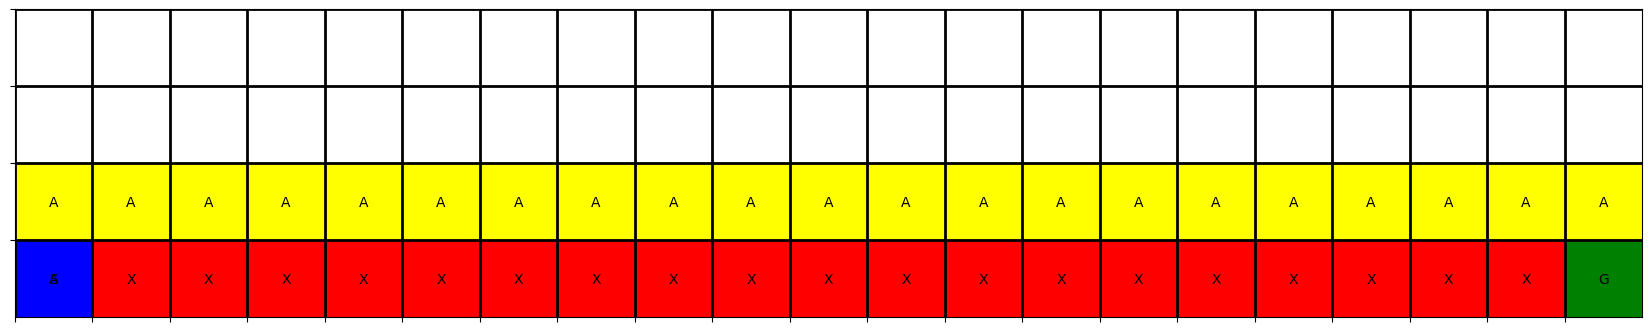
\includegraphics[width=\textwidth]{image/R2.4.png}
        \caption{\scriptsize Optimal path under Q-Learning \(\epsilon=0.3\)}
    \end{minipage}
\end{figure}

\subsubsection{Comparison in Different Environments}
The introduction of a snake pit had a minimal impact on SARSA but significantly affected Q-Learning. This difference highlights the varying adaptability of the two algorithms to changes in environmental complexity and unforeseen obstacles.

\begin{figure}[ht]
    \centering
    \begin{minipage}[b]{0.48\textwidth}
        \centering
        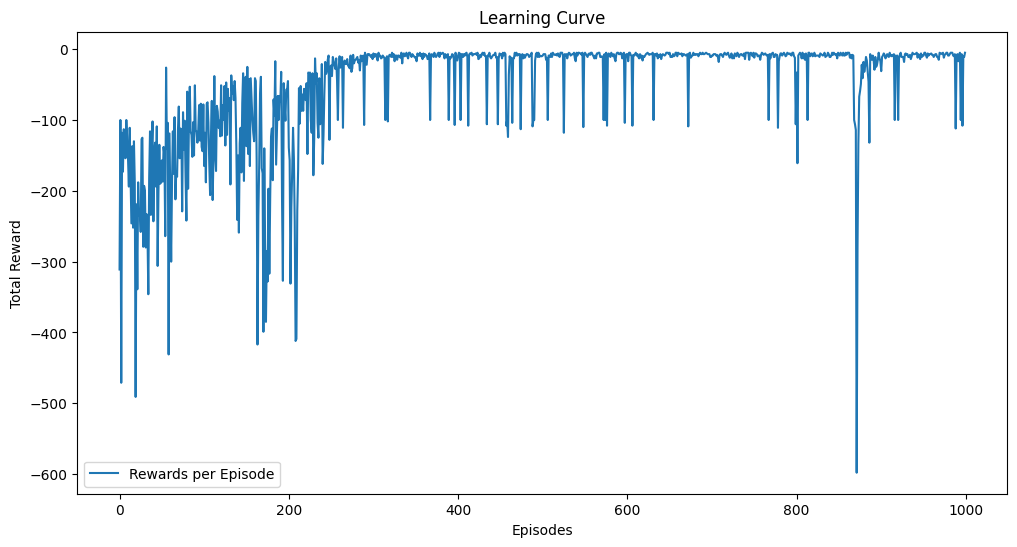
\includegraphics[width=\textwidth]{image/L3.1.png}
        \caption{\scriptsize Learning curves for SARSA, Snake pit}
        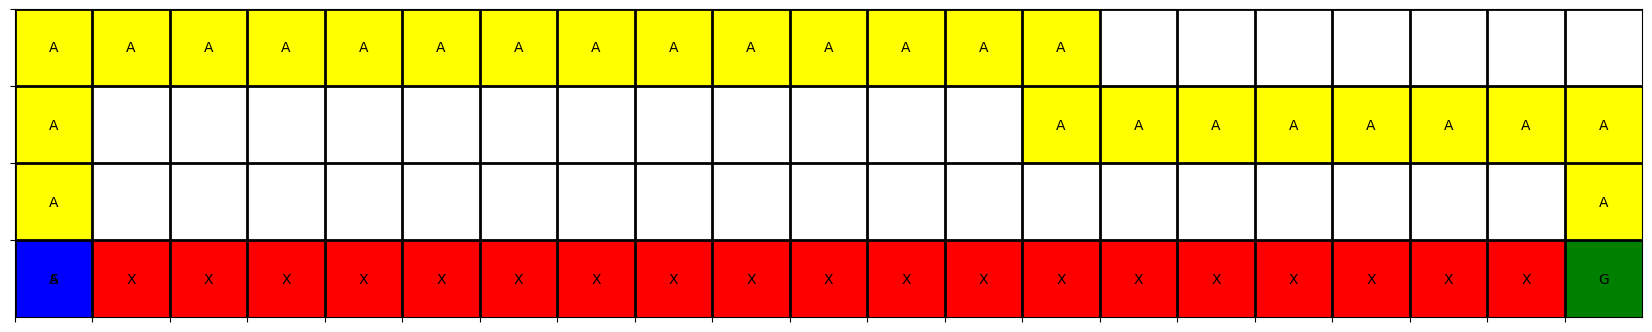
\includegraphics[width=\textwidth]{image/R3.1.png}
        \caption{\scriptsize Optimal path under SARSA, Snake pit}
    \end{minipage}
    \hfill
    \begin{minipage}[b]{0.48\textwidth}
        \centering
        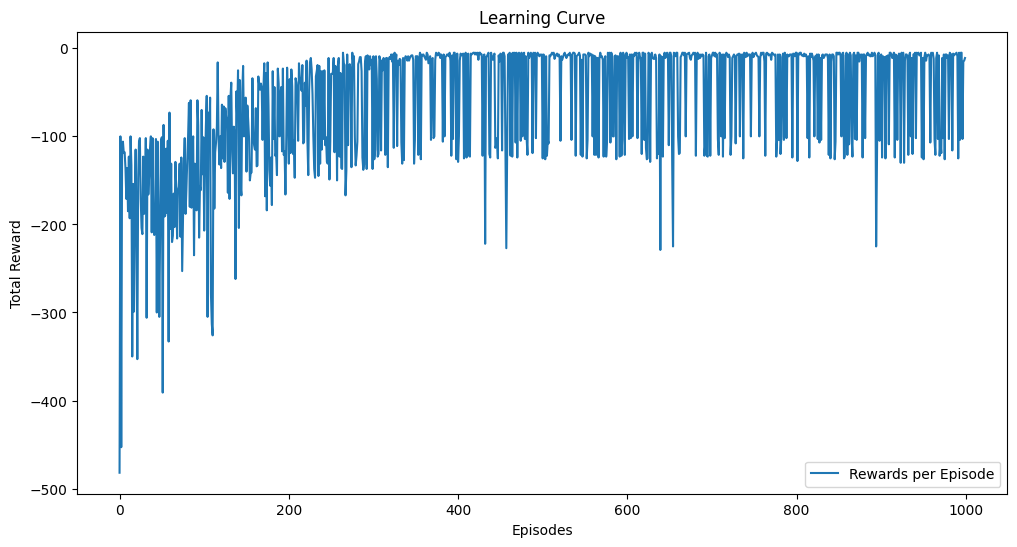
\includegraphics[width=\textwidth]{image/L3.2.png}
        \caption{\scriptsize Learning curves for Q-Learning, Snake pit}
        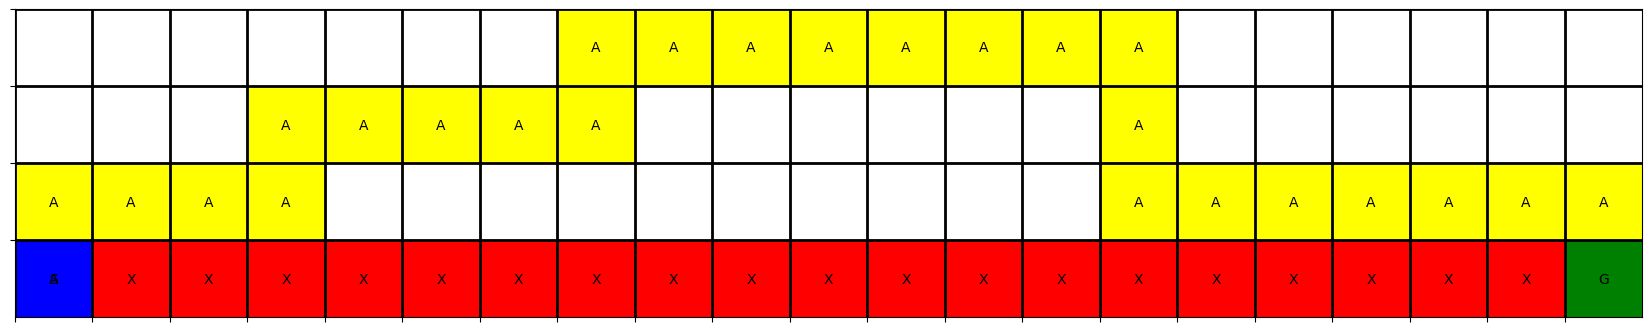
\includegraphics[width=\textwidth]{image/R3.2.png}
        \caption{\scriptsize Optimal path under Q-Learning, Snake pit}
    \end{minipage}
\end{figure}

\subsection{Conclusion}

This study shows how SARSA and Q-Learning behave differently under various conditions. SARSA generally takes safer paths, showing steady progress, while Q-Learning aims for the best possible paths but can be more unpredictable. Changing the exploration rates affected how quickly and smoothly the algorithms learned. Also, adding a snake pit to the environment challenged the algorithms differently, pointing out how each adapts to new challenges. These results underline the need to choose and fine-tune algorithms thoughtfully for different situations in reinforcement learning.

\end{document}
